\section{Abstract}

The main objective of our project is to be able to make a 360-degrees video representation of any object. To do this, a camera will have to takes photos of the object you want to represent at regular intervals. This object will be placed on a turntable. A micro controller named STM32 will have to manage the rotation of the turntable but also the triggering of photos. The user can set the number of photos to be taken for a complete revolution of the turntable in order to obtain a more or less precise rendering. 
\newline
In a first time,  we will explain why we realized it and remind all the specifications of the project. After we will discuss about the improvements of the project since the presentation that we realised in english classroom. 


\section {Why make a 360-degrees representation of an object ?  }

My buddy, Frédéric JENN ALET and me are impassioned by the photography. Frédéric loves takes photos and videos, he's equipped with a Canon DSLR (digital single lens reflex). Personaly. I'm equiped with a Nikon DSLR and I love take sky and stars pitcures. 
In electronics systems classroom of the SME Master, we had to make a project with an STM32. So we decided to make a link between photography and electronic. 

\section{What are the possibles implementations}

Our project can be used in several applications. For exemple in architecture or product design because you need to modelize mock-up in 360 degrees to make behavior studys.
In this part, we will speak about the main application, marketing. 

\subsection{Marketing implementation}
\begin{figure}[h]
    \centering
    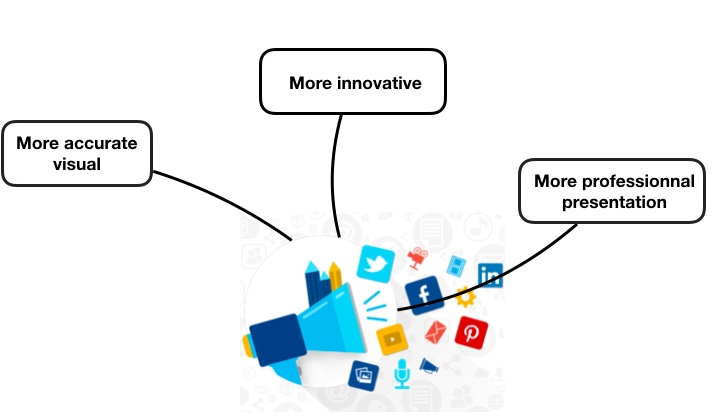
\includegraphics[scale=0.4]{img/marketing.png}\\% Include a department/university logo - this will require the graphicx package
    \caption{Marketing application}
    \label{fig:LogoTachyssema}
  \end{figure}

  Marketing is a very interesting application because, today, more and more devices are sold on websites. Costumers can't see the product with their owns eyes. It can be a problem because they want to know as much informations as possible to be sure the device is a good case or no. 
  With our product, costumers will still not able to see the product with their own eyes, but they will able to see a more precise render in 360 degrees. They will have more confidence and the seller will increase the chances to make sales.  

  Indeed, our project let the seller to create a more accurate, innovative and professionnal visual of their products. 

\section {Advancement since the english presentation  } 

With Frédéric, we divided this part. He will indroduce the first part of the improvements that we have realised since our english presentation in his repport and I will present the others parts. 

\subsection {What is an Human Machine Interface } 

An HMI for Human Machine Interface is a system witch make a link between an user and an other system. It can be composed by  sowtware or hardware components. ( The picture below is an exemple of an HMI that I've realized in my company). 

\begin{figure}[h]
    \centering
    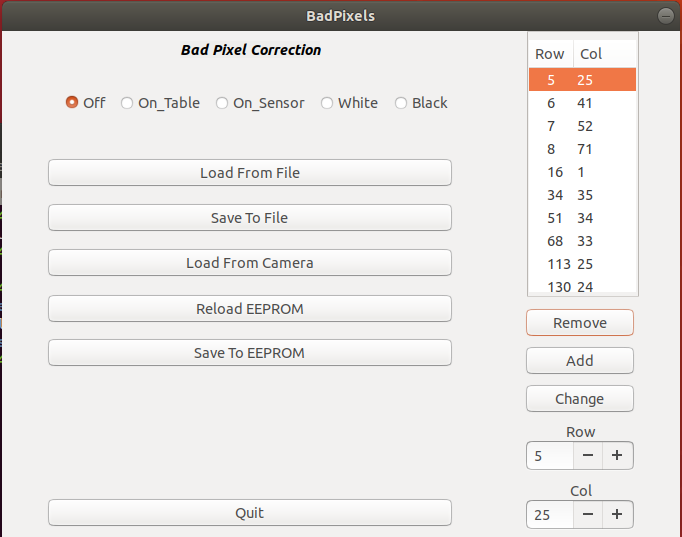
\includegraphics[scale=0.35]{img/IHM.png}\\% Include a department/university logo - this will require the graphicx package
    \caption{Exemple of an HMI}
    \label{fig:LogoTachyssema}
  \end{figure}

  The user can interact with the system with buttons. For exemple, when the user click on a button, a specific command is sending to the system. Also the system can communicate with the user and sends commands to the user. For exemple it can contain status informations about the system. 

\subsection {Human machine interface with LCD screen } 

In a first time, we realized a HMI on a LCD screen on our system. The HMI let us to know the evolution of the number of photos captures remaining before the end of the revolution.

It is very usefull to us because without this HMI, we can't know when the render is done ! 
\newpage

\begin{figure}[h]
  \centering
  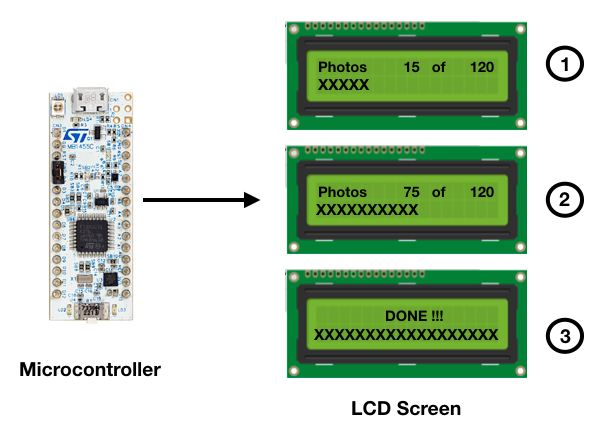
\includegraphics[scale=0.45]{img/LCD_IHM.png}\\% Include a department/university logo - this will require the graphicx package
  \caption{HMI with LCD Screen }
  \label{fig:LogoTachyssema}
\end{figure}

As you can see on the above picture, the LCD screen is composed of 2 lines. The first line shows us the advancement of the render. The second line is loading bar witch is updated. 
\subsection {Human machine interface on a computer  } 

After realized the first LCD HMI, we decided to make an other, with more functionalities. The previous just let us to saw the advancement but this one is a solution to have a real monitoring of the project.  

\subsubsection {Specifications  } 

This Human Machine Interface will communicate with a computer to the communication will be possible in 2 ways. On a first hand the user will can make a configuration of the project and on an other hand, the microcontroller will send data to computer. 
The HMI must is comply with this specifications : 
\newline
\begin{itemize}
  \item The microcontroller will send the advancement of the render.
  \item The user can Stop, start and restart the project.
  \item The user can set the number of photos taken for one revolution of the turntable.
  \item The user is alert when all the photos are taken. 
  \end{itemize}


  \subsubsection {Implementation } 

After describe the specifications, we developped the program on the computer. To build it,  we maked code in C language. The program is able to communicate with the STM32 by a serial line witch is a USB communication. 
\newpage

\begin{figure}[h]
    \centering
    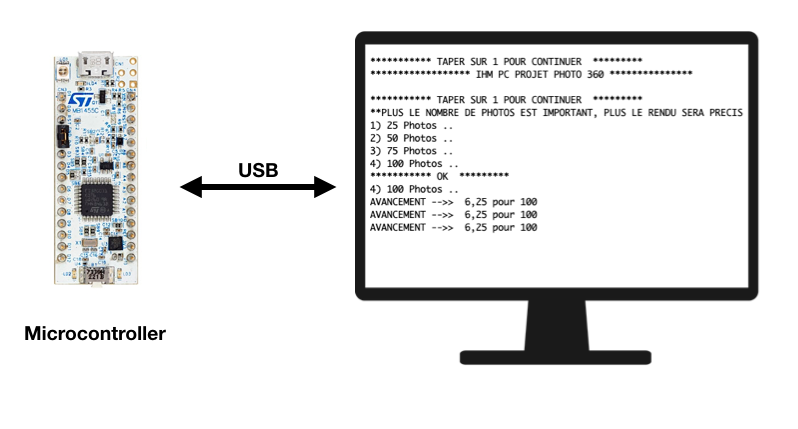
\includegraphics[scale=0.4]{img/IHM_PC.png}\\% Include a department/university logo - this will require the graphicx package
    \caption{Marketing application}
    \label{fig:LogoTachyssema}
  \end{figure}

  Above, you can see the HMI running on a computer. First the user should write '1'. After the microcontroller ask the user to select how many photos he want to make the render. After enter a valid choice, the user can see the advancement of the render. Once the render is finished, the user is alert with a signal. 

\section {Conclusion } 

In this report, I have introduce to you few aspects of the advancement of our project since the english presentation. Today the project is finished. You can check our work by watching this video : \url{https://www.youtube.com/watch?v=agmECTL7zs8&feature=youtube.be }. 
We have realised all the specifications that we had fixed, so the project is done. 
This projet allows us to devellop many technicals skills. For exemple, we realized the mecanical part, which consisted in manufacturing a personnalized turntable. Also, we develloped electronical skills, where we could make the study of a microcontroller which where the STM32. 
Finally, we learned to realized images processing, which allow us to realized a rendering of a 360 degrees object.

